\documentclass[10pt, letterpaper]{article}

% Packages:
\usepackage[
    ignoreheadfoot, % set margins without considering header and footer
    top=2 cm, % seperation between body and page edge from the top
    bottom=2 cm, % seperation between body and page edge from the bottom
    left=2 cm, % seperation between body and page edge from the left
    right=2 cm, % seperation between body and page edge from the right
    footskip=1.0 cm, % seperation between body and footer
    % showframe % for debugging 
]{geometry} % for adjusting page geometry
\usepackage[explicit]{titlesec} % for customizing section titles
\usepackage{tabularx} % for making tables with fixed width columns
\usepackage{array} % tabularx requires this
\usepackage[dvipsnames]{xcolor} % for coloring text
\definecolor{primaryColor}{RGB}{0, 79, 144} % define primary color
\usepackage{enumitem} % for customizing lists
\usepackage{fontawesome5} % for using icons
\usepackage{amsmath} % for math
\usepackage[
    pdftitle={John Doe's CV},
    pdfauthor={John Doe},
    pdfcreator={LaTeX with RenderCV},
    colorlinks=true,
    urlcolor=primaryColor
]{hyperref} % for links, metadata and bookmarks
\usepackage[pscoord]{eso-pic} % for floating text on the page
\usepackage{calc} % for calculating lengths
\usepackage{bookmark} % for bookmarks
\usepackage{lastpage} % for getting the total number of pages
\usepackage{changepage} % for one column entries (adjustwidth environment)
\usepackage{paracol} % for two and three column entries
\usepackage{ifthen} % for conditional statements
\usepackage{needspace} % for avoiding page brake right after the section title
\usepackage{iftex} % check if engine is pdflatex, xetex or luatex
% Ensure that generate pdf is machine readable/ATS parsable:
\ifPDFTeX
    \input{glyphtounicode}
    \pdfgentounicode=1
    \usepackage[T1]{fontenc}
    \usepackage[utf8]{inputenc}
    \usepackage{lmodern}
\fi
\usepackage[default, type1]{sourcesanspro} 
\usepackage{graphicx} % for the profile picture

% Some settings:
\AtBeginEnvironment{adjustwidth}{\partopsep0pt} % remove space before adjustwidth environment
\pagestyle{empty} % no header or footer
\setcounter{secnumdepth}{0} % no section numbering
\setlength{\parindent}{0pt} % no indentation
\setlength{\topskip}{0pt} % no top skip
\setlength{\columnsep}{0.15cm} % set column seperation
\makeatletter
\let\ps@customFooterStyle\ps@plain % Copy the plain style to customFooterStyle
\patchcmd{\ps@customFooterStyle}{\thepage}{
    \color{gray}\textit{\small John Doe - Page \thepage{} of \pageref*{LastPage}}
}{}{} % replace number by desired string
\makeatother
\pagestyle{customFooterStyle}

\titleformat{\section}{
    % avoid page braking right after the section title
    \needspace{4\baselineskip}
    % make the font size of the section title large and color it with the primary color
    \Large\color{primaryColor}
}{
}{
}{
    % print bold title, give 0.15 cm space and draw a line of 0.8 pt thickness
    % from the end of the title to the end of the body
    \textbf{#1}\hspace{0.15cm}\titlerule[0.8pt]\hspace{-0.1cm}
}[] % section title formatting

\titlespacing{\section}{
    % left space:
    -1pt
}{
    % top space:
    0.3 cm
}{
    % bottom space:
    0.2 cm
} % section title spacing

% \renewcommand\labelitemi{$\vcenter{\hbox{\small$\bullet$}}$} % custom bullet points
\newenvironment{highlights}{
    \begin{itemize}[
        topsep=0.10 cm,
        parsep=0.10 cm,
        partopsep=0pt,
        itemsep=0pt,
        leftmargin=0.4 cm + 10pt
    ]
}{
    \end{itemize}
} % new environment for highlights

\newenvironment{highlightsforbulletentries}{
    \begin{itemize}[
        topsep=0.10 cm,
        parsep=0.10 cm,
        partopsep=0pt,
        itemsep=0pt,
        leftmargin=10pt
    ]
}{
    \end{itemize}
} % new environment for highlights for bullet entries


\newenvironment{onecolentry}{
    \begin{adjustwidth}{
        0.2 cm + 0.00001 cm
    }{
        0.2 cm + 0.00001 cm
    }
}{
    \end{adjustwidth}
} % new environment for one column entries

\newenvironment{twocolentry}[2][]{
    \onecolentry
    \def\secondColumn{#2}
    \setcolumnwidth{\fill, 4.5 cm}
    \begin{paracol}{2}
}{
    \switchcolumn \raggedleft \secondColumn
    \end{paracol}
    \endonecolentry
} % new environment for two column entries

\newenvironment{threecolentry}[3][]{
    \onecolentry
    \def\thirdColumn{#3}
    \setcolumnwidth{1 cm, \fill, 4.5 cm}
    \begin{paracol}{3}
    {\raggedright #2} \switchcolumn
}{
    \switchcolumn \raggedleft \thirdColumn
    \end{paracol}
    \endonecolentry
} % new environment for three column entries

\newenvironment{header}{
    \setlength{\topsep}{0pt}\par\kern\topsep\centering\color{primaryColor}\linespread{1.5}
}{
    \par\kern\topsep
} % new environment for the header

\newcommand{\placelastupdatedtext}{% \placetextbox{<horizontal pos>}{<vertical pos>}{<stuff>}
  \AddToShipoutPictureFG*{% Add <stuff> to current page foreground
    \put(
        \LenToUnit{\paperwidth-2 cm-0.2 cm+0.05cm},
        \LenToUnit{\paperheight-1.0 cm}
    ){\vtop{{\null}\makebox[0pt][c]{
        \small\color{gray}\textit{Last updated in January 2024}\hspace{\widthof{Last updated in January 2024}}
    }}}%
  }%
}%

\newenvironment{twocolheadercontainer}[2][]{
    \onecolentry
    \def\secondColumn{#2}
    \setcolumnwidth{\fill, 0.2\linewidth}
    \begin{paracol}{2}
}{
    \switchcolumn \raggedleft \secondColumn
    \end{paracol}
    \endonecolentry
} % new environment for headers with profile pictures

% save the original href command in a new command:
\let\hrefWithoutArrow\href

% new command for external links:
\renewcommand{\href}[2]{\hrefWithoutArrow{#1}{\ifthenelse{\equal{#2}{}}{ }{#2 }\raisebox{.15ex}{\footnotesize \faExternalLink*}}}


\begin{document}
    \newcommand{\AND}{\unskip
        \cleaders\copy\ANDbox\hskip\wd\ANDbox
        \ignorespaces
    }
    \newsavebox\ANDbox
    \sbox\ANDbox{}

    \placelastupdatedtext

    \begin{twocolheadercontainer}{
        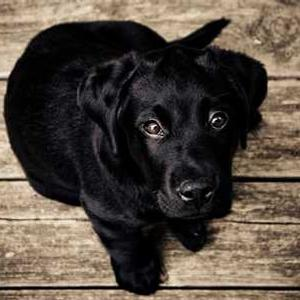
\includegraphics[width=\linewidth]{profile_picture.png}

    }
    \begin{header}
        \raggedright
        \fontsize{30 pt}{30 pt}
        \textbf{John Doe}

        \vspace{0.3 cm}

        \normalsize
        \mbox{{\footnotesize\faMapMarker*}\hspace*{0.13cm}Istanbul, Turkey}%
        \kern 0.25 cm%
        \AND%
        \kern 0.25 cm%
        \mbox{\hrefWithoutArrow{mailto:john_doe@example.com}{{\footnotesize\faEnvelope[regular]}\hspace*{0.13cm}john\_doe@example.com}}%
        \kern 0.25 cm%
        \AND%
        \kern 0.25 cm%
        \mbox{\hrefWithoutArrow{tel:+90-541-999-99-99}{{\footnotesize\faPhone*}\hspace*{0.13cm}0541 999 99 99}}%
        \kern 0.25 cm%
        \AND%
        \kern 0.25 cm%
        \mbox{\hrefWithoutArrow{https://example.com/}{{\footnotesize\faLink}\hspace*{0.13cm}example.com}}%
        \kern 0.25 cm%
        \AND%
        \kern 0.25 cm%
        \mbox{\hrefWithoutArrow{https://linkedin.com/in/johndoe}{{\footnotesize\faLinkedinIn}\hspace*{0.13cm}johndoe}}%
        \kern 0.25 cm%
        \AND%
        \kern 0.25 cm%
        \mbox{\hrefWithoutArrow{https://github.com/johndoe}{{\footnotesize\faGithub}\hspace*{0.13cm}johndoe}}%
        \kern 0.25 cm%
        \AND%
        \kern 0.25 cm%
        \mbox{\hrefWithoutArrow{https://instagram.com/johndoe}{{\footnotesize\faInstagram}\hspace*{0.13cm}johndoe}}%
        \kern 0.25 cm%
        \AND%
        \kern 0.25 cm%
        \mbox{\hrefWithoutArrow{https://orcid.org/0000-0000-0000-0000}{{\footnotesize\faOrcid}\hspace*{0.13cm}0000-0000-0000-0000}}%
        \kern 0.25 cm%
        \AND%
        \kern 0.25 cm%
        \mbox{\hrefWithoutArrow{https://scholar.google.com/citations?user=F8IyYrQAAAAJ}{{\footnotesize\faGraduationCap}\hspace*{0.13cm}Google Scholar}}%
        \kern 0.25 cm%
        \AND%
        \kern 0.25 cm%
        \mbox{\hrefWithoutArrow{https://example.com/@johndoe}{{\footnotesize\faMastodon}\hspace*{0.13cm}@johndoe@example.com}}%
        \kern 0.25 cm%
        \AND%
        \kern 0.25 cm%
        \mbox{\hrefWithoutArrow{https://stackoverflow.com/users/12323/johndoe}{{\footnotesize\faStackOverflow}\hspace*{0.13cm}johndoe}}%
        \kern 0.25 cm%
        \AND%
        \kern 0.25 cm%
        \mbox{\hrefWithoutArrow{https://gitlab.com/johndoe}{{\footnotesize\faGitlab}\hspace*{0.13cm}johndoe}}%
        \kern 0.25 cm%
        \AND%
        \kern 0.25 cm%
        \mbox{\hrefWithoutArrow{https://researchgate.net/profile/johndoe}{{\footnotesize\faResearchgate}\hspace*{0.13cm}johndoe}}%
        \kern 0.25 cm%
        \AND%
        \kern 0.25 cm%
        \mbox{\hrefWithoutArrow{https://youtube.com/@johndoe}{{\footnotesize\faYoutube}\hspace*{0.13cm}johndoe}}%
        \kern 0.25 cm%
        \AND%
        \kern 0.25 cm%
        \mbox{\hrefWithoutArrow{https://t.me/johndoe}{{\footnotesize\faTelegram}\hspace*{0.13cm}johndoe}}%
    \end{header}
    \end{twocolheadercontainer}

    \vspace{0.3 cm - 0.3 cm}


    \section{Text Entries}



        
        \begin{onecolentry}
            This is a \textit{TextEntry}. It is only a text and can be useful for sections like \textbf{Summary}. To showcase the TextEntry completely, this sentence is added, but it doesn't contain any information.
        \end{onecolentry}

        \vspace{0.2 cm}

        \begin{onecolentry}
            This is a \textit{TextEntry}. It is only a text and can be useful for sections like \textbf{Summary}. To showcase the TextEntry completely, this sentence is added, but it doesn't contain any information.
        \end{onecolentry}

        \vspace{0.2 cm}

        \begin{onecolentry}
            This is a \textit{TextEntry}. It is only a text and can be useful for sections like \textbf{Summary}. To showcase the TextEntry completely, this sentence is added, but it doesn't contain any information.
        \end{onecolentry}


    
    \section{Bullet Entries}

    \begin{onecolentry}
        \begin{highlightsforbulletentries}


        \item This is a bullet entry.

        \item This is a bullet entry.


        \end{highlightsforbulletentries}
    \end{onecolentry}

    \section{Publication Entries}



        
        \begin{samepage}
            \begin{onecolentry}
                \textbf{Magneto-Thermal Thin Shell Approximation for 3D Finite Element Analysis of No-Insulation Coils}

                \vspace{0.10 cm}

                \mbox{J. Doe}, \mbox{\textbf{\textit{H. Tom}}}, \mbox{S. Doe}, \mbox{A. Andsurname}, \mbox{S. Doe}, \mbox{A. Andsurname}, \mbox{S. Doe}, \mbox{A. Andsurname}, \mbox{S. Doe}, \mbox{A. Andsurname}
            \end{onecolentry}
        \end{samepage}

        \vspace{0.2 cm}

        \begin{samepage}
            \begin{onecolentry}
                \textbf{Magneto-Thermal Thin Shell Approximation for 3D Finite Element Analysis of No-Insulation Coils}

                \vspace{0.10 cm}

                \mbox{J. Doe}, \mbox{\textbf{\textit{H. Tom}}}, \mbox{S. Doe}, \mbox{A. Andsurname}, \mbox{S. Doe}, \mbox{A. Andsurname}, \mbox{S. Doe}, \mbox{A. Andsurname}, \mbox{S. Doe}, \mbox{A. Andsurname}
                \vspace{0.10 cm}

        \href{https://doi.org/10.1007/978-3-319-69626-3_101-1}{10.1007/978-3-319-69626-3\_101-1}
            \end{onecolentry}
        \end{samepage}

        \vspace{0.2 cm}

        \begin{samepage}
            \begin{onecolentry}
                \textbf{Magneto-Thermal Thin Shell Approximation for 3D Finite Element Analysis of No-Insulation Coils}

                \vspace{0.10 cm}

                \mbox{J. Doe}, \mbox{\textbf{\textit{H. Tom}}}, \mbox{S. Doe}, \mbox{A. Andsurname}, \mbox{S. Doe}, \mbox{A. Andsurname}, \mbox{S. Doe}, \mbox{A. Andsurname}, \mbox{S. Doe}, \mbox{A. Andsurname}
                \vspace{0.10 cm}

        \href{https://example.com}{example.com}    \end{onecolentry}
        \end{samepage}

        \vspace{0.2 cm}

        \begin{samepage}
            \begin{onecolentry}
                \textbf{Magneto-Thermal Thin Shell Approximation for 3D Finite Element Analysis of No-Insulation Coils}

                \vspace{0.10 cm}

                \mbox{J. Doe}, \mbox{\textbf{\textit{H. Tom}}}, \mbox{S. Doe}, \mbox{A. Andsurname}, \mbox{S. Doe}, \mbox{A. Andsurname}, \mbox{S. Doe}, \mbox{A. Andsurname}, \mbox{S. Doe}, \mbox{A. Andsurname}
                \vspace{0.10 cm}

        IEEE Transactions on Applied Superconductivity    \end{onecolentry}
        \end{samepage}

        \vspace{0.2 cm}

        \begin{samepage}
            \begin{twocolentry}{
                Sept 2021
            }
                \textbf{Magneto-Thermal Thin Shell Approximation for 3D Finite Element Analysis of No-Insulation Coils}

                \vspace{0.10 cm}

                \mbox{J. Doe}, \mbox{\textbf{\textit{H. Tom}}}, \mbox{S. Doe}, \mbox{A. Andsurname}, \mbox{S. Doe}, \mbox{A. Andsurname}, \mbox{S. Doe}, \mbox{A. Andsurname}, \mbox{S. Doe}, \mbox{A. Andsurname}
            \end{twocolentry}
        \end{samepage}

        \vspace{0.2 cm}

        \begin{samepage}
            \begin{onecolentry}
                \textbf{Magneto-Thermal Thin Shell Approximation for 3D Finite Element Analysis of No-Insulation Coils}

                \vspace{0.10 cm}

                \mbox{J. Doe}, \mbox{\textbf{\textit{H. Tom}}}, \mbox{S. Doe}, \mbox{A. Andsurname}, \mbox{S. Doe}, \mbox{A. Andsurname}, \mbox{S. Doe}, \mbox{A. Andsurname}, \mbox{S. Doe}, \mbox{A. Andsurname}
                \vspace{0.10 cm}

        \href{https://doi.org/10.1007/978-3-319-69626-3_101-1}{10.1007/978-3-319-69626-3\_101-1}
            \end{onecolentry}
        \end{samepage}

        \vspace{0.2 cm}

        \begin{samepage}
            \begin{onecolentry}
                \textbf{Magneto-Thermal Thin Shell Approximation for 3D Finite Element Analysis of No-Insulation Coils}

                \vspace{0.10 cm}

                \mbox{J. Doe}, \mbox{\textbf{\textit{H. Tom}}}, \mbox{S. Doe}, \mbox{A. Andsurname}, \mbox{S. Doe}, \mbox{A. Andsurname}, \mbox{S. Doe}, \mbox{A. Andsurname}, \mbox{S. Doe}, \mbox{A. Andsurname}
                \vspace{0.10 cm}

        \href{https://doi.org/10.1007/978-3-319-69626-3_101-1}{10.1007/978-3-319-69626-3\_101-1}
         (IEEE Transactions on Applied Superconductivity)    \end{onecolentry}
        \end{samepage}

        \vspace{0.2 cm}

        \begin{samepage}
            \begin{twocolentry}{
                Sept 2021
            }
                \textbf{Magneto-Thermal Thin Shell Approximation for 3D Finite Element Analysis of No-Insulation Coils}

                \vspace{0.10 cm}

                \mbox{J. Doe}, \mbox{\textbf{\textit{H. Tom}}}, \mbox{S. Doe}, \mbox{A. Andsurname}, \mbox{S. Doe}, \mbox{A. Andsurname}, \mbox{S. Doe}, \mbox{A. Andsurname}, \mbox{S. Doe}, \mbox{A. Andsurname}
                \vspace{0.10 cm}

        \href{https://doi.org/10.1007/978-3-319-69626-3_101-1}{10.1007/978-3-319-69626-3\_101-1}
            \end{twocolentry}
        \end{samepage}

        \vspace{0.2 cm}

        \begin{samepage}
            \begin{onecolentry}
                \textbf{Magneto-Thermal Thin Shell Approximation for 3D Finite Element Analysis of No-Insulation Coils}

                \vspace{0.10 cm}

                \mbox{J. Doe}, \mbox{\textbf{\textit{H. Tom}}}, \mbox{S. Doe}, \mbox{A. Andsurname}, \mbox{S. Doe}, \mbox{A. Andsurname}, \mbox{S. Doe}, \mbox{A. Andsurname}, \mbox{S. Doe}, \mbox{A. Andsurname}
                \vspace{0.10 cm}

        \href{https://example.com}{example.com} (IEEE Transactions on Applied Superconductivity)    \end{onecolentry}
        \end{samepage}

        \vspace{0.2 cm}

        \begin{samepage}
            \begin{twocolentry}{
                Sept 2021
            }
                \textbf{Magneto-Thermal Thin Shell Approximation for 3D Finite Element Analysis of No-Insulation Coils}

                \vspace{0.10 cm}

                \mbox{J. Doe}, \mbox{\textbf{\textit{H. Tom}}}, \mbox{S. Doe}, \mbox{A. Andsurname}, \mbox{S. Doe}, \mbox{A. Andsurname}, \mbox{S. Doe}, \mbox{A. Andsurname}, \mbox{S. Doe}, \mbox{A. Andsurname}
                \vspace{0.10 cm}

        \href{https://example.com}{example.com}    \end{twocolentry}
        \end{samepage}

        \vspace{0.2 cm}

        \begin{samepage}
            \begin{twocolentry}{
                Sept 2021
            }
                \textbf{Magneto-Thermal Thin Shell Approximation for 3D Finite Element Analysis of No-Insulation Coils}

                \vspace{0.10 cm}

                \mbox{J. Doe}, \mbox{\textbf{\textit{H. Tom}}}, \mbox{S. Doe}, \mbox{A. Andsurname}, \mbox{S. Doe}, \mbox{A. Andsurname}, \mbox{S. Doe}, \mbox{A. Andsurname}, \mbox{S. Doe}, \mbox{A. Andsurname}
                \vspace{0.10 cm}

        IEEE Transactions on Applied Superconductivity    \end{twocolentry}
        \end{samepage}

        \vspace{0.2 cm}

        \begin{samepage}
            \begin{onecolentry}
                \textbf{Magneto-Thermal Thin Shell Approximation for 3D Finite Element Analysis of No-Insulation Coils}

                \vspace{0.10 cm}

                \mbox{J. Doe}, \mbox{\textbf{\textit{H. Tom}}}, \mbox{S. Doe}, \mbox{A. Andsurname}, \mbox{S. Doe}, \mbox{A. Andsurname}, \mbox{S. Doe}, \mbox{A. Andsurname}, \mbox{S. Doe}, \mbox{A. Andsurname}
                \vspace{0.10 cm}

        \href{https://doi.org/10.1007/978-3-319-69626-3_101-1}{10.1007/978-3-319-69626-3\_101-1}
         (IEEE Transactions on Applied Superconductivity)    \end{onecolentry}
        \end{samepage}

        \vspace{0.2 cm}

        \begin{samepage}
            \begin{twocolentry}{
                Sept 2021
            }
                \textbf{Magneto-Thermal Thin Shell Approximation for 3D Finite Element Analysis of No-Insulation Coils}

                \vspace{0.10 cm}

                \mbox{J. Doe}, \mbox{\textbf{\textit{H. Tom}}}, \mbox{S. Doe}, \mbox{A. Andsurname}, \mbox{S. Doe}, \mbox{A. Andsurname}, \mbox{S. Doe}, \mbox{A. Andsurname}, \mbox{S. Doe}, \mbox{A. Andsurname}
                \vspace{0.10 cm}

        \href{https://doi.org/10.1007/978-3-319-69626-3_101-1}{10.1007/978-3-319-69626-3\_101-1}
            \end{twocolentry}
        \end{samepage}

        \vspace{0.2 cm}

        \begin{samepage}
            \begin{twocolentry}{
                Sept 2021
            }
                \textbf{Magneto-Thermal Thin Shell Approximation for 3D Finite Element Analysis of No-Insulation Coils}

                \vspace{0.10 cm}

                \mbox{J. Doe}, \mbox{\textbf{\textit{H. Tom}}}, \mbox{S. Doe}, \mbox{A. Andsurname}, \mbox{S. Doe}, \mbox{A. Andsurname}, \mbox{S. Doe}, \mbox{A. Andsurname}, \mbox{S. Doe}, \mbox{A. Andsurname}
                \vspace{0.10 cm}

        \href{https://doi.org/10.1007/978-3-319-69626-3_101-1}{10.1007/978-3-319-69626-3\_101-1}
         (IEEE Transactions on Applied Superconductivity)    \end{twocolentry}
        \end{samepage}

        \vspace{0.2 cm}

        \begin{samepage}
            \begin{twocolentry}{
                Sept 2021
            }
                \textbf{Magneto-Thermal Thin Shell Approximation for 3D Finite Element Analysis of No-Insulation Coils}

                \vspace{0.10 cm}

                \mbox{J. Doe}, \mbox{\textbf{\textit{H. Tom}}}, \mbox{S. Doe}, \mbox{A. Andsurname}, \mbox{S. Doe}, \mbox{A. Andsurname}, \mbox{S. Doe}, \mbox{A. Andsurname}, \mbox{S. Doe}, \mbox{A. Andsurname}
                \vspace{0.10 cm}

        \href{https://example.com}{example.com} (IEEE Transactions on Applied Superconductivity)    \end{twocolentry}
        \end{samepage}

        \vspace{0.2 cm}

        \begin{samepage}
            \begin{twocolentry}{
                Sept 2021
            }
                \textbf{Magneto-Thermal Thin Shell Approximation for 3D Finite Element Analysis of No-Insulation Coils}

                \vspace{0.10 cm}

                \mbox{J. Doe}, \mbox{\textbf{\textit{H. Tom}}}, \mbox{S. Doe}, \mbox{A. Andsurname}, \mbox{S. Doe}, \mbox{A. Andsurname}, \mbox{S. Doe}, \mbox{A. Andsurname}, \mbox{S. Doe}, \mbox{A. Andsurname}
                \vspace{0.10 cm}

        \href{https://doi.org/10.1007/978-3-319-69626-3_101-1}{10.1007/978-3-319-69626-3\_101-1}
         (IEEE Transactions on Applied Superconductivity)    \end{twocolentry}
        \end{samepage}


    
    \section{Experience Entries}



        
        \begin{onecolentry}
            \textbf{Some \textnormal{Company}}, Software Engineer
        \end{onecolentry}


        \vspace{0.2 cm}

        \begin{twocolentry}{
            Sept 2021
        }
            \textbf{Some \textnormal{Company}}, Software Engineer
        \end{twocolentry}


        \vspace{0.2 cm}

        \begin{twocolentry}{
            Istanbul, Turkey
        }
            \textbf{Some \textnormal{Company}}, Software Engineer
        \end{twocolentry}


        \vspace{0.2 cm}

        \begin{twocolentry}{
            Sept 2015 – present
        }
            \textbf{Some \textnormal{Company}}, Software Engineer
        \end{twocolentry}


        \vspace{0.2 cm}

        \begin{twocolentry}{
            June 2020
        }
            \textbf{Some \textnormal{Company}}, Software Engineer
        \end{twocolentry}


        \vspace{0.2 cm}

        \begin{onecolentry}
            \textbf{Some \textnormal{Company}}, Software Engineer
            \begin{highlights}
                \item Did \textit{this} and this is a \textbf{bold} \href{https://example.com}{link}. But I must explain to you how all this mistaken idea of denouncing pleasure and praising pain was born and I will give you a complete account of the system, and expound the actual teachings of the great explorer of the truth, the master-builder of human happiness. No one rejects, dislikes, or avoids pleasure itself, because it is pleasure, but because those who do not know how to pursue pleasure rationally encounter consequences that are extremely painful.
                \item Did that. Nor again is there anyone who loves or pursues or desires to obtain pain of itself, because it is pain, but because occasionally circumstances occur in which toil and pain can procure him some great pleasure.
            \end{highlights}
        \end{onecolentry}


        \vspace{0.2 cm}

        \begin{twocolentry}{
            Istanbul, Turkey

        Sept 2021
        }
            \textbf{Some \textnormal{Company}}, Software Engineer
        \end{twocolentry}


        \vspace{0.2 cm}

        \begin{twocolentry}{
            Sept 2021
        }
            \textbf{Some \textnormal{Company}}, Software Engineer
        \end{twocolentry}


        \vspace{0.2 cm}

        \begin{twocolentry}{
            Sept 2021
        }
            \textbf{Some \textnormal{Company}}, Software Engineer
        \end{twocolentry}


        \vspace{0.2 cm}

        \begin{twocolentry}{
            Sept 2021
        }
            \textbf{Some \textnormal{Company}}, Software Engineer
            \begin{highlights}
                \item Did \textit{this} and this is a \textbf{bold} \href{https://example.com}{link}. But I must explain to you how all this mistaken idea of denouncing pleasure and praising pain was born and I will give you a complete account of the system, and expound the actual teachings of the great explorer of the truth, the master-builder of human happiness. No one rejects, dislikes, or avoids pleasure itself, because it is pleasure, but because those who do not know how to pursue pleasure rationally encounter consequences that are extremely painful.
                \item Did that. Nor again is there anyone who loves or pursues or desires to obtain pain of itself, because it is pain, but because occasionally circumstances occur in which toil and pain can procure him some great pleasure.
            \end{highlights}
        \end{twocolentry}


        \vspace{0.2 cm}

        \begin{twocolentry}{
            Istanbul, Turkey

        Sept 2015 – present
        }
            \textbf{Some \textnormal{Company}}, Software Engineer
        \end{twocolentry}


        \vspace{0.2 cm}

        \begin{twocolentry}{
            Istanbul, Turkey

        June 2020
        }
            \textbf{Some \textnormal{Company}}, Software Engineer
        \end{twocolentry}


        \vspace{0.2 cm}

        \begin{twocolentry}{
            Istanbul, Turkey
        }
            \textbf{Some \textnormal{Company}}, Software Engineer
            \begin{highlights}
                \item Did \textit{this} and this is a \textbf{bold} \href{https://example.com}{link}. But I must explain to you how all this mistaken idea of denouncing pleasure and praising pain was born and I will give you a complete account of the system, and expound the actual teachings of the great explorer of the truth, the master-builder of human happiness. No one rejects, dislikes, or avoids pleasure itself, because it is pleasure, but because those who do not know how to pursue pleasure rationally encounter consequences that are extremely painful.
                \item Did that. Nor again is there anyone who loves or pursues or desires to obtain pain of itself, because it is pain, but because occasionally circumstances occur in which toil and pain can procure him some great pleasure.
            \end{highlights}
        \end{twocolentry}


        \vspace{0.2 cm}

        \begin{twocolentry}{
            Sept 2015 – June 2020
        }
            \textbf{Some \textnormal{Company}}, Software Engineer
        \end{twocolentry}


        \vspace{0.2 cm}

        \begin{twocolentry}{
            Sept 2015 – present
        }
            \textbf{Some \textnormal{Company}}, Software Engineer
            \begin{highlights}
                \item Did \textit{this} and this is a \textbf{bold} \href{https://example.com}{link}. But I must explain to you how all this mistaken idea of denouncing pleasure and praising pain was born and I will give you a complete account of the system, and expound the actual teachings of the great explorer of the truth, the master-builder of human happiness. No one rejects, dislikes, or avoids pleasure itself, because it is pleasure, but because those who do not know how to pursue pleasure rationally encounter consequences that are extremely painful.
                \item Did that. Nor again is there anyone who loves or pursues or desires to obtain pain of itself, because it is pain, but because occasionally circumstances occur in which toil and pain can procure him some great pleasure.
            \end{highlights}
        \end{twocolentry}


        \vspace{0.2 cm}

        \begin{twocolentry}{
            June 2020
        }
            \textbf{Some \textnormal{Company}}, Software Engineer
            \begin{highlights}
                \item Did \textit{this} and this is a \textbf{bold} \href{https://example.com}{link}. But I must explain to you how all this mistaken idea of denouncing pleasure and praising pain was born and I will give you a complete account of the system, and expound the actual teachings of the great explorer of the truth, the master-builder of human happiness. No one rejects, dislikes, or avoids pleasure itself, because it is pleasure, but because those who do not know how to pursue pleasure rationally encounter consequences that are extremely painful.
                \item Did that. Nor again is there anyone who loves or pursues or desires to obtain pain of itself, because it is pain, but because occasionally circumstances occur in which toil and pain can procure him some great pleasure.
            \end{highlights}
        \end{twocolentry}


        \vspace{0.2 cm}

        \begin{twocolentry}{
            Istanbul, Turkey

        Sept 2021
        }
            \textbf{Some \textnormal{Company}}, Software Engineer
        \end{twocolentry}


        \vspace{0.2 cm}

        \begin{twocolentry}{
            Istanbul, Turkey

        Sept 2021
        }
            \textbf{Some \textnormal{Company}}, Software Engineer
        \end{twocolentry}


        \vspace{0.2 cm}

        \begin{twocolentry}{
            Istanbul, Turkey

        Sept 2021
        }
            \textbf{Some \textnormal{Company}}, Software Engineer
            \begin{highlights}
                \item Did \textit{this} and this is a \textbf{bold} \href{https://example.com}{link}. But I must explain to you how all this mistaken idea of denouncing pleasure and praising pain was born and I will give you a complete account of the system, and expound the actual teachings of the great explorer of the truth, the master-builder of human happiness. No one rejects, dislikes, or avoids pleasure itself, because it is pleasure, but because those who do not know how to pursue pleasure rationally encounter consequences that are extremely painful.
                \item Did that. Nor again is there anyone who loves or pursues or desires to obtain pain of itself, because it is pain, but because occasionally circumstances occur in which toil and pain can procure him some great pleasure.
            \end{highlights}
        \end{twocolentry}


        \vspace{0.2 cm}

        \begin{twocolentry}{
            Sept 2021
        }
            \textbf{Some \textnormal{Company}}, Software Engineer
        \end{twocolentry}


        \vspace{0.2 cm}

        \begin{twocolentry}{
            Sept 2021
        }
            \textbf{Some \textnormal{Company}}, Software Engineer
            \begin{highlights}
                \item Did \textit{this} and this is a \textbf{bold} \href{https://example.com}{link}. But I must explain to you how all this mistaken idea of denouncing pleasure and praising pain was born and I will give you a complete account of the system, and expound the actual teachings of the great explorer of the truth, the master-builder of human happiness. No one rejects, dislikes, or avoids pleasure itself, because it is pleasure, but because those who do not know how to pursue pleasure rationally encounter consequences that are extremely painful.
                \item Did that. Nor again is there anyone who loves or pursues or desires to obtain pain of itself, because it is pain, but because occasionally circumstances occur in which toil and pain can procure him some great pleasure.
            \end{highlights}
        \end{twocolentry}


        \vspace{0.2 cm}

        \begin{twocolentry}{
            Sept 2021
        }
            \textbf{Some \textnormal{Company}}, Software Engineer
            \begin{highlights}
                \item Did \textit{this} and this is a \textbf{bold} \href{https://example.com}{link}. But I must explain to you how all this mistaken idea of denouncing pleasure and praising pain was born and I will give you a complete account of the system, and expound the actual teachings of the great explorer of the truth, the master-builder of human happiness. No one rejects, dislikes, or avoids pleasure itself, because it is pleasure, but because those who do not know how to pursue pleasure rationally encounter consequences that are extremely painful.
                \item Did that. Nor again is there anyone who loves or pursues or desires to obtain pain of itself, because it is pain, but because occasionally circumstances occur in which toil and pain can procure him some great pleasure.
            \end{highlights}
        \end{twocolentry}


        \vspace{0.2 cm}

        \begin{twocolentry}{
            Istanbul, Turkey

        Sept 2015 – June 2020
        }
            \textbf{Some \textnormal{Company}}, Software Engineer
        \end{twocolentry}


        \vspace{0.2 cm}

        \begin{twocolentry}{
            Istanbul, Turkey

        Sept 2015 – present
        }
            \textbf{Some \textnormal{Company}}, Software Engineer
            \begin{highlights}
                \item Did \textit{this} and this is a \textbf{bold} \href{https://example.com}{link}. But I must explain to you how all this mistaken idea of denouncing pleasure and praising pain was born and I will give you a complete account of the system, and expound the actual teachings of the great explorer of the truth, the master-builder of human happiness. No one rejects, dislikes, or avoids pleasure itself, because it is pleasure, but because those who do not know how to pursue pleasure rationally encounter consequences that are extremely painful.
                \item Did that. Nor again is there anyone who loves or pursues or desires to obtain pain of itself, because it is pain, but because occasionally circumstances occur in which toil and pain can procure him some great pleasure.
            \end{highlights}
        \end{twocolentry}


        \vspace{0.2 cm}

        \begin{twocolentry}{
            Istanbul, Turkey

        June 2020
        }
            \textbf{Some \textnormal{Company}}, Software Engineer
            \begin{highlights}
                \item Did \textit{this} and this is a \textbf{bold} \href{https://example.com}{link}. But I must explain to you how all this mistaken idea of denouncing pleasure and praising pain was born and I will give you a complete account of the system, and expound the actual teachings of the great explorer of the truth, the master-builder of human happiness. No one rejects, dislikes, or avoids pleasure itself, because it is pleasure, but because those who do not know how to pursue pleasure rationally encounter consequences that are extremely painful.
                \item Did that. Nor again is there anyone who loves or pursues or desires to obtain pain of itself, because it is pain, but because occasionally circumstances occur in which toil and pain can procure him some great pleasure.
            \end{highlights}
        \end{twocolentry}


        \vspace{0.2 cm}

        \begin{twocolentry}{
            Sept 2015 – June 2020
        }
            \textbf{Some \textnormal{Company}}, Software Engineer
            \begin{highlights}
                \item Did \textit{this} and this is a \textbf{bold} \href{https://example.com}{link}. But I must explain to you how all this mistaken idea of denouncing pleasure and praising pain was born and I will give you a complete account of the system, and expound the actual teachings of the great explorer of the truth, the master-builder of human happiness. No one rejects, dislikes, or avoids pleasure itself, because it is pleasure, but because those who do not know how to pursue pleasure rationally encounter consequences that are extremely painful.
                \item Did that. Nor again is there anyone who loves or pursues or desires to obtain pain of itself, because it is pain, but because occasionally circumstances occur in which toil and pain can procure him some great pleasure.
            \end{highlights}
        \end{twocolentry}


        \vspace{0.2 cm}

        \begin{twocolentry}{
            Istanbul, Turkey

        Sept 2021
        }
            \textbf{Some \textnormal{Company}}, Software Engineer
        \end{twocolentry}


        \vspace{0.2 cm}

        \begin{twocolentry}{
            Istanbul, Turkey

        Sept 2021
        }
            \textbf{Some \textnormal{Company}}, Software Engineer
            \begin{highlights}
                \item Did \textit{this} and this is a \textbf{bold} \href{https://example.com}{link}. But I must explain to you how all this mistaken idea of denouncing pleasure and praising pain was born and I will give you a complete account of the system, and expound the actual teachings of the great explorer of the truth, the master-builder of human happiness. No one rejects, dislikes, or avoids pleasure itself, because it is pleasure, but because those who do not know how to pursue pleasure rationally encounter consequences that are extremely painful.
                \item Did that. Nor again is there anyone who loves or pursues or desires to obtain pain of itself, because it is pain, but because occasionally circumstances occur in which toil and pain can procure him some great pleasure.
            \end{highlights}
        \end{twocolentry}


        \vspace{0.2 cm}

        \begin{twocolentry}{
            Istanbul, Turkey

        Sept 2021
        }
            \textbf{Some \textnormal{Company}}, Software Engineer
            \begin{highlights}
                \item Did \textit{this} and this is a \textbf{bold} \href{https://example.com}{link}. But I must explain to you how all this mistaken idea of denouncing pleasure and praising pain was born and I will give you a complete account of the system, and expound the actual teachings of the great explorer of the truth, the master-builder of human happiness. No one rejects, dislikes, or avoids pleasure itself, because it is pleasure, but because those who do not know how to pursue pleasure rationally encounter consequences that are extremely painful.
                \item Did that. Nor again is there anyone who loves or pursues or desires to obtain pain of itself, because it is pain, but because occasionally circumstances occur in which toil and pain can procure him some great pleasure.
            \end{highlights}
        \end{twocolentry}


        \vspace{0.2 cm}

        \begin{twocolentry}{
            Sept 2021
        }
            \textbf{Some \textnormal{Company}}, Software Engineer
            \begin{highlights}
                \item Did \textit{this} and this is a \textbf{bold} \href{https://example.com}{link}. But I must explain to you how all this mistaken idea of denouncing pleasure and praising pain was born and I will give you a complete account of the system, and expound the actual teachings of the great explorer of the truth, the master-builder of human happiness. No one rejects, dislikes, or avoids pleasure itself, because it is pleasure, but because those who do not know how to pursue pleasure rationally encounter consequences that are extremely painful.
                \item Did that. Nor again is there anyone who loves or pursues or desires to obtain pain of itself, because it is pain, but because occasionally circumstances occur in which toil and pain can procure him some great pleasure.
            \end{highlights}
        \end{twocolentry}


        \vspace{0.2 cm}

        \begin{twocolentry}{
            Istanbul, Turkey

        Sept 2015 – June 2020
        }
            \textbf{Some \textnormal{Company}}, Software Engineer
            \begin{highlights}
                \item Did \textit{this} and this is a \textbf{bold} \href{https://example.com}{link}. But I must explain to you how all this mistaken idea of denouncing pleasure and praising pain was born and I will give you a complete account of the system, and expound the actual teachings of the great explorer of the truth, the master-builder of human happiness. No one rejects, dislikes, or avoids pleasure itself, because it is pleasure, but because those who do not know how to pursue pleasure rationally encounter consequences that are extremely painful.
                \item Did that. Nor again is there anyone who loves or pursues or desires to obtain pain of itself, because it is pain, but because occasionally circumstances occur in which toil and pain can procure him some great pleasure.
            \end{highlights}
        \end{twocolentry}


        \vspace{0.2 cm}

        \begin{twocolentry}{
            Istanbul, Turkey

        Sept 2021
        }
            \textbf{Some \textnormal{Company}}, Software Engineer
            \begin{highlights}
                \item Did \textit{this} and this is a \textbf{bold} \href{https://example.com}{link}. But I must explain to you how all this mistaken idea of denouncing pleasure and praising pain was born and I will give you a complete account of the system, and expound the actual teachings of the great explorer of the truth, the master-builder of human happiness. No one rejects, dislikes, or avoids pleasure itself, because it is pleasure, but because those who do not know how to pursue pleasure rationally encounter consequences that are extremely painful.
                \item Did that. Nor again is there anyone who loves or pursues or desires to obtain pain of itself, because it is pain, but because occasionally circumstances occur in which toil and pain can procure him some great pleasure.
            \end{highlights}
        \end{twocolentry}



    
    \section{Education Entries}



        
        \begin{threecolentry}{\textbf{}}{
            
        }
            \textbf{Boğaziçi University}, Mechanical Engineering
        \end{threecolentry}

        \vspace{0.2 cm}

        \begin{threecolentry}{\textbf{BS}}{
            
        }
            \textbf{Boğaziçi University}, Mechanical Engineering
        \end{threecolentry}

        \vspace{0.2 cm}

        \begin{threecolentry}{\textbf{}}{
            Sept 2021
        }
            \textbf{Boğaziçi University}, Mechanical Engineering
        \end{threecolentry}

        \vspace{0.2 cm}

        \begin{threecolentry}{\textbf{}}{
            Istanbul, Turkey
        }
            \textbf{Boğaziçi University}, Mechanical Engineering
        \end{threecolentry}

        \vspace{0.2 cm}

        \begin{threecolentry}{\textbf{}}{
            Sept 2015 – present
        }
            \textbf{Boğaziçi University}, Mechanical Engineering
        \end{threecolentry}

        \vspace{0.2 cm}

        \begin{threecolentry}{\textbf{}}{
            June 2020
        }
            \textbf{Boğaziçi University}, Mechanical Engineering
        \end{threecolentry}

        \vspace{0.2 cm}

        \begin{threecolentry}{\textbf{}}{
            
        }
            \textbf{Boğaziçi University}, Mechanical Engineering
            \begin{highlights}
                \item Did \textit{this} and this is a \textbf{bold} \href{https://example.com}{link}. But I must explain to you how all this mistaken idea of denouncing pleasure and praising pain was born and I will give you a complete account of the system, and expound the actual teachings of the great explorer of the truth, the master-builder of human happiness. No one rejects, dislikes, or avoids pleasure itself, because it is pleasure, but because those who do not know how to pursue pleasure rationally encounter consequences that are extremely painful.
                \item Did that. Nor again is there anyone who loves or pursues or desires to obtain pain of itself, because it is pain, but because occasionally circumstances occur in which toil and pain can procure him some great pleasure.
            \end{highlights}
        \end{threecolentry}

        \vspace{0.2 cm}

        \begin{threecolentry}{\textbf{BS}}{
            Sept 2021
        }
            \textbf{Boğaziçi University}, Mechanical Engineering
        \end{threecolentry}

        \vspace{0.2 cm}

        \begin{threecolentry}{\textbf{BS}}{
            Istanbul, Turkey
        }
            \textbf{Boğaziçi University}, Mechanical Engineering
        \end{threecolentry}

        \vspace{0.2 cm}

        \begin{threecolentry}{\textbf{BS}}{
            Sept 2015 – present
        }
            \textbf{Boğaziçi University}, Mechanical Engineering
        \end{threecolentry}

        \vspace{0.2 cm}

        \begin{threecolentry}{\textbf{BS}}{
            June 2020
        }
            \textbf{Boğaziçi University}, Mechanical Engineering
        \end{threecolentry}

        \vspace{0.2 cm}

        \begin{threecolentry}{\textbf{BS}}{
            
        }
            \textbf{Boğaziçi University}, Mechanical Engineering
            \begin{highlights}
                \item Did \textit{this} and this is a \textbf{bold} \href{https://example.com}{link}. But I must explain to you how all this mistaken idea of denouncing pleasure and praising pain was born and I will give you a complete account of the system, and expound the actual teachings of the great explorer of the truth, the master-builder of human happiness. No one rejects, dislikes, or avoids pleasure itself, because it is pleasure, but because those who do not know how to pursue pleasure rationally encounter consequences that are extremely painful.
                \item Did that. Nor again is there anyone who loves or pursues or desires to obtain pain of itself, because it is pain, but because occasionally circumstances occur in which toil and pain can procure him some great pleasure.
            \end{highlights}
        \end{threecolentry}

        \vspace{0.2 cm}

        \begin{threecolentry}{\textbf{}}{
            Istanbul, Turkey

        Sept 2021
        }
            \textbf{Boğaziçi University}, Mechanical Engineering
        \end{threecolentry}

        \vspace{0.2 cm}

        \begin{threecolentry}{\textbf{}}{
            Sept 2021
        }
            \textbf{Boğaziçi University}, Mechanical Engineering
        \end{threecolentry}

        \vspace{0.2 cm}

        \begin{threecolentry}{\textbf{}}{
            Sept 2021
        }
            \textbf{Boğaziçi University}, Mechanical Engineering
        \end{threecolentry}

        \vspace{0.2 cm}

        \begin{threecolentry}{\textbf{}}{
            Sept 2021
        }
            \textbf{Boğaziçi University}, Mechanical Engineering
            \begin{highlights}
                \item Did \textit{this} and this is a \textbf{bold} \href{https://example.com}{link}. But I must explain to you how all this mistaken idea of denouncing pleasure and praising pain was born and I will give you a complete account of the system, and expound the actual teachings of the great explorer of the truth, the master-builder of human happiness. No one rejects, dislikes, or avoids pleasure itself, because it is pleasure, but because those who do not know how to pursue pleasure rationally encounter consequences that are extremely painful.
                \item Did that. Nor again is there anyone who loves or pursues or desires to obtain pain of itself, because it is pain, but because occasionally circumstances occur in which toil and pain can procure him some great pleasure.
            \end{highlights}
        \end{threecolentry}

        \vspace{0.2 cm}

        \begin{threecolentry}{\textbf{}}{
            Istanbul, Turkey

        Sept 2015 – present
        }
            \textbf{Boğaziçi University}, Mechanical Engineering
        \end{threecolentry}

        \vspace{0.2 cm}

        \begin{threecolentry}{\textbf{}}{
            Istanbul, Turkey

        June 2020
        }
            \textbf{Boğaziçi University}, Mechanical Engineering
        \end{threecolentry}

        \vspace{0.2 cm}

        \begin{threecolentry}{\textbf{}}{
            Istanbul, Turkey
        }
            \textbf{Boğaziçi University}, Mechanical Engineering
            \begin{highlights}
                \item Did \textit{this} and this is a \textbf{bold} \href{https://example.com}{link}. But I must explain to you how all this mistaken idea of denouncing pleasure and praising pain was born and I will give you a complete account of the system, and expound the actual teachings of the great explorer of the truth, the master-builder of human happiness. No one rejects, dislikes, or avoids pleasure itself, because it is pleasure, but because those who do not know how to pursue pleasure rationally encounter consequences that are extremely painful.
                \item Did that. Nor again is there anyone who loves or pursues or desires to obtain pain of itself, because it is pain, but because occasionally circumstances occur in which toil and pain can procure him some great pleasure.
            \end{highlights}
        \end{threecolentry}

        \vspace{0.2 cm}

        \begin{threecolentry}{\textbf{}}{
            Sept 2015 – June 2020
        }
            \textbf{Boğaziçi University}, Mechanical Engineering
        \end{threecolentry}

        \vspace{0.2 cm}

        \begin{threecolentry}{\textbf{}}{
            Sept 2015 – present
        }
            \textbf{Boğaziçi University}, Mechanical Engineering
            \begin{highlights}
                \item Did \textit{this} and this is a \textbf{bold} \href{https://example.com}{link}. But I must explain to you how all this mistaken idea of denouncing pleasure and praising pain was born and I will give you a complete account of the system, and expound the actual teachings of the great explorer of the truth, the master-builder of human happiness. No one rejects, dislikes, or avoids pleasure itself, because it is pleasure, but because those who do not know how to pursue pleasure rationally encounter consequences that are extremely painful.
                \item Did that. Nor again is there anyone who loves or pursues or desires to obtain pain of itself, because it is pain, but because occasionally circumstances occur in which toil and pain can procure him some great pleasure.
            \end{highlights}
        \end{threecolentry}

        \vspace{0.2 cm}

        \begin{threecolentry}{\textbf{}}{
            June 2020
        }
            \textbf{Boğaziçi University}, Mechanical Engineering
            \begin{highlights}
                \item Did \textit{this} and this is a \textbf{bold} \href{https://example.com}{link}. But I must explain to you how all this mistaken idea of denouncing pleasure and praising pain was born and I will give you a complete account of the system, and expound the actual teachings of the great explorer of the truth, the master-builder of human happiness. No one rejects, dislikes, or avoids pleasure itself, because it is pleasure, but because those who do not know how to pursue pleasure rationally encounter consequences that are extremely painful.
                \item Did that. Nor again is there anyone who loves or pursues or desires to obtain pain of itself, because it is pain, but because occasionally circumstances occur in which toil and pain can procure him some great pleasure.
            \end{highlights}
        \end{threecolentry}

        \vspace{0.2 cm}

        \begin{threecolentry}{\textbf{BS}}{
            Istanbul, Turkey

        Sept 2021
        }
            \textbf{Boğaziçi University}, Mechanical Engineering
        \end{threecolentry}

        \vspace{0.2 cm}

        \begin{threecolentry}{\textbf{BS}}{
            Sept 2021
        }
            \textbf{Boğaziçi University}, Mechanical Engineering
        \end{threecolentry}

        \vspace{0.2 cm}

        \begin{threecolentry}{\textbf{BS}}{
            Sept 2021
        }
            \textbf{Boğaziçi University}, Mechanical Engineering
        \end{threecolentry}

        \vspace{0.2 cm}

        \begin{threecolentry}{\textbf{BS}}{
            Sept 2021
        }
            \textbf{Boğaziçi University}, Mechanical Engineering
            \begin{highlights}
                \item Did \textit{this} and this is a \textbf{bold} \href{https://example.com}{link}. But I must explain to you how all this mistaken idea of denouncing pleasure and praising pain was born and I will give you a complete account of the system, and expound the actual teachings of the great explorer of the truth, the master-builder of human happiness. No one rejects, dislikes, or avoids pleasure itself, because it is pleasure, but because those who do not know how to pursue pleasure rationally encounter consequences that are extremely painful.
                \item Did that. Nor again is there anyone who loves or pursues or desires to obtain pain of itself, because it is pain, but because occasionally circumstances occur in which toil and pain can procure him some great pleasure.
            \end{highlights}
        \end{threecolentry}

        \vspace{0.2 cm}

        \begin{threecolentry}{\textbf{BS}}{
            Istanbul, Turkey

        Sept 2015 – present
        }
            \textbf{Boğaziçi University}, Mechanical Engineering
        \end{threecolentry}

        \vspace{0.2 cm}

        \begin{threecolentry}{\textbf{BS}}{
            Istanbul, Turkey

        June 2020
        }
            \textbf{Boğaziçi University}, Mechanical Engineering
        \end{threecolentry}

        \vspace{0.2 cm}

        \begin{threecolentry}{\textbf{BS}}{
            Istanbul, Turkey
        }
            \textbf{Boğaziçi University}, Mechanical Engineering
            \begin{highlights}
                \item Did \textit{this} and this is a \textbf{bold} \href{https://example.com}{link}. But I must explain to you how all this mistaken idea of denouncing pleasure and praising pain was born and I will give you a complete account of the system, and expound the actual teachings of the great explorer of the truth, the master-builder of human happiness. No one rejects, dislikes, or avoids pleasure itself, because it is pleasure, but because those who do not know how to pursue pleasure rationally encounter consequences that are extremely painful.
                \item Did that. Nor again is there anyone who loves or pursues or desires to obtain pain of itself, because it is pain, but because occasionally circumstances occur in which toil and pain can procure him some great pleasure.
            \end{highlights}
        \end{threecolentry}

        \vspace{0.2 cm}

        \begin{threecolentry}{\textbf{BS}}{
            Sept 2015 – June 2020
        }
            \textbf{Boğaziçi University}, Mechanical Engineering
        \end{threecolentry}

        \vspace{0.2 cm}

        \begin{threecolentry}{\textbf{BS}}{
            Sept 2015 – present
        }
            \textbf{Boğaziçi University}, Mechanical Engineering
            \begin{highlights}
                \item Did \textit{this} and this is a \textbf{bold} \href{https://example.com}{link}. But I must explain to you how all this mistaken idea of denouncing pleasure and praising pain was born and I will give you a complete account of the system, and expound the actual teachings of the great explorer of the truth, the master-builder of human happiness. No one rejects, dislikes, or avoids pleasure itself, because it is pleasure, but because those who do not know how to pursue pleasure rationally encounter consequences that are extremely painful.
                \item Did that. Nor again is there anyone who loves or pursues or desires to obtain pain of itself, because it is pain, but because occasionally circumstances occur in which toil and pain can procure him some great pleasure.
            \end{highlights}
        \end{threecolentry}

        \vspace{0.2 cm}

        \begin{threecolentry}{\textbf{BS}}{
            June 2020
        }
            \textbf{Boğaziçi University}, Mechanical Engineering
            \begin{highlights}
                \item Did \textit{this} and this is a \textbf{bold} \href{https://example.com}{link}. But I must explain to you how all this mistaken idea of denouncing pleasure and praising pain was born and I will give you a complete account of the system, and expound the actual teachings of the great explorer of the truth, the master-builder of human happiness. No one rejects, dislikes, or avoids pleasure itself, because it is pleasure, but because those who do not know how to pursue pleasure rationally encounter consequences that are extremely painful.
                \item Did that. Nor again is there anyone who loves or pursues or desires to obtain pain of itself, because it is pain, but because occasionally circumstances occur in which toil and pain can procure him some great pleasure.
            \end{highlights}
        \end{threecolentry}

        \vspace{0.2 cm}

        \begin{threecolentry}{\textbf{}}{
            Istanbul, Turkey

        Sept 2021
        }
            \textbf{Boğaziçi University}, Mechanical Engineering
        \end{threecolentry}

        \vspace{0.2 cm}

        \begin{threecolentry}{\textbf{}}{
            Istanbul, Turkey

        Sept 2021
        }
            \textbf{Boğaziçi University}, Mechanical Engineering
        \end{threecolentry}

        \vspace{0.2 cm}

        \begin{threecolentry}{\textbf{}}{
            Istanbul, Turkey

        Sept 2021
        }
            \textbf{Boğaziçi University}, Mechanical Engineering
            \begin{highlights}
                \item Did \textit{this} and this is a \textbf{bold} \href{https://example.com}{link}. But I must explain to you how all this mistaken idea of denouncing pleasure and praising pain was born and I will give you a complete account of the system, and expound the actual teachings of the great explorer of the truth, the master-builder of human happiness. No one rejects, dislikes, or avoids pleasure itself, because it is pleasure, but because those who do not know how to pursue pleasure rationally encounter consequences that are extremely painful.
                \item Did that. Nor again is there anyone who loves or pursues or desires to obtain pain of itself, because it is pain, but because occasionally circumstances occur in which toil and pain can procure him some great pleasure.
            \end{highlights}
        \end{threecolentry}

        \vspace{0.2 cm}

        \begin{threecolentry}{\textbf{}}{
            Sept 2021
        }
            \textbf{Boğaziçi University}, Mechanical Engineering
        \end{threecolentry}

        \vspace{0.2 cm}

        \begin{threecolentry}{\textbf{}}{
            Sept 2021
        }
            \textbf{Boğaziçi University}, Mechanical Engineering
            \begin{highlights}
                \item Did \textit{this} and this is a \textbf{bold} \href{https://example.com}{link}. But I must explain to you how all this mistaken idea of denouncing pleasure and praising pain was born and I will give you a complete account of the system, and expound the actual teachings of the great explorer of the truth, the master-builder of human happiness. No one rejects, dislikes, or avoids pleasure itself, because it is pleasure, but because those who do not know how to pursue pleasure rationally encounter consequences that are extremely painful.
                \item Did that. Nor again is there anyone who loves or pursues or desires to obtain pain of itself, because it is pain, but because occasionally circumstances occur in which toil and pain can procure him some great pleasure.
            \end{highlights}
        \end{threecolentry}

        \vspace{0.2 cm}

        \begin{threecolentry}{\textbf{}}{
            Sept 2021
        }
            \textbf{Boğaziçi University}, Mechanical Engineering
            \begin{highlights}
                \item Did \textit{this} and this is a \textbf{bold} \href{https://example.com}{link}. But I must explain to you how all this mistaken idea of denouncing pleasure and praising pain was born and I will give you a complete account of the system, and expound the actual teachings of the great explorer of the truth, the master-builder of human happiness. No one rejects, dislikes, or avoids pleasure itself, because it is pleasure, but because those who do not know how to pursue pleasure rationally encounter consequences that are extremely painful.
                \item Did that. Nor again is there anyone who loves or pursues or desires to obtain pain of itself, because it is pain, but because occasionally circumstances occur in which toil and pain can procure him some great pleasure.
            \end{highlights}
        \end{threecolentry}

        \vspace{0.2 cm}

        \begin{threecolentry}{\textbf{}}{
            Istanbul, Turkey

        Sept 2015 – June 2020
        }
            \textbf{Boğaziçi University}, Mechanical Engineering
        \end{threecolentry}

        \vspace{0.2 cm}

        \begin{threecolentry}{\textbf{}}{
            Istanbul, Turkey

        Sept 2015 – present
        }
            \textbf{Boğaziçi University}, Mechanical Engineering
            \begin{highlights}
                \item Did \textit{this} and this is a \textbf{bold} \href{https://example.com}{link}. But I must explain to you how all this mistaken idea of denouncing pleasure and praising pain was born and I will give you a complete account of the system, and expound the actual teachings of the great explorer of the truth, the master-builder of human happiness. No one rejects, dislikes, or avoids pleasure itself, because it is pleasure, but because those who do not know how to pursue pleasure rationally encounter consequences that are extremely painful.
                \item Did that. Nor again is there anyone who loves or pursues or desires to obtain pain of itself, because it is pain, but because occasionally circumstances occur in which toil and pain can procure him some great pleasure.
            \end{highlights}
        \end{threecolentry}

        \vspace{0.2 cm}

        \begin{threecolentry}{\textbf{}}{
            Istanbul, Turkey

        June 2020
        }
            \textbf{Boğaziçi University}, Mechanical Engineering
            \begin{highlights}
                \item Did \textit{this} and this is a \textbf{bold} \href{https://example.com}{link}. But I must explain to you how all this mistaken idea of denouncing pleasure and praising pain was born and I will give you a complete account of the system, and expound the actual teachings of the great explorer of the truth, the master-builder of human happiness. No one rejects, dislikes, or avoids pleasure itself, because it is pleasure, but because those who do not know how to pursue pleasure rationally encounter consequences that are extremely painful.
                \item Did that. Nor again is there anyone who loves or pursues or desires to obtain pain of itself, because it is pain, but because occasionally circumstances occur in which toil and pain can procure him some great pleasure.
            \end{highlights}
        \end{threecolentry}

        \vspace{0.2 cm}

        \begin{threecolentry}{\textbf{}}{
            Sept 2015 – June 2020
        }
            \textbf{Boğaziçi University}, Mechanical Engineering
            \begin{highlights}
                \item Did \textit{this} and this is a \textbf{bold} \href{https://example.com}{link}. But I must explain to you how all this mistaken idea of denouncing pleasure and praising pain was born and I will give you a complete account of the system, and expound the actual teachings of the great explorer of the truth, the master-builder of human happiness. No one rejects, dislikes, or avoids pleasure itself, because it is pleasure, but because those who do not know how to pursue pleasure rationally encounter consequences that are extremely painful.
                \item Did that. Nor again is there anyone who loves or pursues or desires to obtain pain of itself, because it is pain, but because occasionally circumstances occur in which toil and pain can procure him some great pleasure.
            \end{highlights}
        \end{threecolentry}

        \vspace{0.2 cm}

        \begin{threecolentry}{\textbf{BS}}{
            Istanbul, Turkey

        Sept 2021
        }
            \textbf{Boğaziçi University}, Mechanical Engineering
        \end{threecolentry}

        \vspace{0.2 cm}

        \begin{threecolentry}{\textbf{BS}}{
            Istanbul, Turkey

        Sept 2021
        }
            \textbf{Boğaziçi University}, Mechanical Engineering
        \end{threecolentry}

        \vspace{0.2 cm}

        \begin{threecolentry}{\textbf{BS}}{
            Istanbul, Turkey

        Sept 2021
        }
            \textbf{Boğaziçi University}, Mechanical Engineering
            \begin{highlights}
                \item Did \textit{this} and this is a \textbf{bold} \href{https://example.com}{link}. But I must explain to you how all this mistaken idea of denouncing pleasure and praising pain was born and I will give you a complete account of the system, and expound the actual teachings of the great explorer of the truth, the master-builder of human happiness. No one rejects, dislikes, or avoids pleasure itself, because it is pleasure, but because those who do not know how to pursue pleasure rationally encounter consequences that are extremely painful.
                \item Did that. Nor again is there anyone who loves or pursues or desires to obtain pain of itself, because it is pain, but because occasionally circumstances occur in which toil and pain can procure him some great pleasure.
            \end{highlights}
        \end{threecolentry}

        \vspace{0.2 cm}

        \begin{threecolentry}{\textbf{BS}}{
            Sept 2021
        }
            \textbf{Boğaziçi University}, Mechanical Engineering
        \end{threecolentry}

        \vspace{0.2 cm}

        \begin{threecolentry}{\textbf{BS}}{
            Sept 2021
        }
            \textbf{Boğaziçi University}, Mechanical Engineering
            \begin{highlights}
                \item Did \textit{this} and this is a \textbf{bold} \href{https://example.com}{link}. But I must explain to you how all this mistaken idea of denouncing pleasure and praising pain was born and I will give you a complete account of the system, and expound the actual teachings of the great explorer of the truth, the master-builder of human happiness. No one rejects, dislikes, or avoids pleasure itself, because it is pleasure, but because those who do not know how to pursue pleasure rationally encounter consequences that are extremely painful.
                \item Did that. Nor again is there anyone who loves or pursues or desires to obtain pain of itself, because it is pain, but because occasionally circumstances occur in which toil and pain can procure him some great pleasure.
            \end{highlights}
        \end{threecolentry}

        \vspace{0.2 cm}

        \begin{threecolentry}{\textbf{BS}}{
            Sept 2021
        }
            \textbf{Boğaziçi University}, Mechanical Engineering
            \begin{highlights}
                \item Did \textit{this} and this is a \textbf{bold} \href{https://example.com}{link}. But I must explain to you how all this mistaken idea of denouncing pleasure and praising pain was born and I will give you a complete account of the system, and expound the actual teachings of the great explorer of the truth, the master-builder of human happiness. No one rejects, dislikes, or avoids pleasure itself, because it is pleasure, but because those who do not know how to pursue pleasure rationally encounter consequences that are extremely painful.
                \item Did that. Nor again is there anyone who loves or pursues or desires to obtain pain of itself, because it is pain, but because occasionally circumstances occur in which toil and pain can procure him some great pleasure.
            \end{highlights}
        \end{threecolentry}

        \vspace{0.2 cm}

        \begin{threecolentry}{\textbf{BS}}{
            Istanbul, Turkey

        Sept 2015 – June 2020
        }
            \textbf{Boğaziçi University}, Mechanical Engineering
        \end{threecolentry}

        \vspace{0.2 cm}

        \begin{threecolentry}{\textbf{BS}}{
            Istanbul, Turkey

        Sept 2015 – present
        }
            \textbf{Boğaziçi University}, Mechanical Engineering
            \begin{highlights}
                \item Did \textit{this} and this is a \textbf{bold} \href{https://example.com}{link}. But I must explain to you how all this mistaken idea of denouncing pleasure and praising pain was born and I will give you a complete account of the system, and expound the actual teachings of the great explorer of the truth, the master-builder of human happiness. No one rejects, dislikes, or avoids pleasure itself, because it is pleasure, but because those who do not know how to pursue pleasure rationally encounter consequences that are extremely painful.
                \item Did that. Nor again is there anyone who loves or pursues or desires to obtain pain of itself, because it is pain, but because occasionally circumstances occur in which toil and pain can procure him some great pleasure.
            \end{highlights}
        \end{threecolentry}

        \vspace{0.2 cm}

        \begin{threecolentry}{\textbf{BS}}{
            Istanbul, Turkey

        June 2020
        }
            \textbf{Boğaziçi University}, Mechanical Engineering
            \begin{highlights}
                \item Did \textit{this} and this is a \textbf{bold} \href{https://example.com}{link}. But I must explain to you how all this mistaken idea of denouncing pleasure and praising pain was born and I will give you a complete account of the system, and expound the actual teachings of the great explorer of the truth, the master-builder of human happiness. No one rejects, dislikes, or avoids pleasure itself, because it is pleasure, but because those who do not know how to pursue pleasure rationally encounter consequences that are extremely painful.
                \item Did that. Nor again is there anyone who loves or pursues or desires to obtain pain of itself, because it is pain, but because occasionally circumstances occur in which toil and pain can procure him some great pleasure.
            \end{highlights}
        \end{threecolentry}

        \vspace{0.2 cm}

        \begin{threecolentry}{\textbf{BS}}{
            Sept 2015 – June 2020
        }
            \textbf{Boğaziçi University}, Mechanical Engineering
            \begin{highlights}
                \item Did \textit{this} and this is a \textbf{bold} \href{https://example.com}{link}. But I must explain to you how all this mistaken idea of denouncing pleasure and praising pain was born and I will give you a complete account of the system, and expound the actual teachings of the great explorer of the truth, the master-builder of human happiness. No one rejects, dislikes, or avoids pleasure itself, because it is pleasure, but because those who do not know how to pursue pleasure rationally encounter consequences that are extremely painful.
                \item Did that. Nor again is there anyone who loves or pursues or desires to obtain pain of itself, because it is pain, but because occasionally circumstances occur in which toil and pain can procure him some great pleasure.
            \end{highlights}
        \end{threecolentry}

        \vspace{0.2 cm}

        \begin{threecolentry}{\textbf{}}{
            Istanbul, Turkey

        Sept 2021
        }
            \textbf{Boğaziçi University}, Mechanical Engineering
        \end{threecolentry}

        \vspace{0.2 cm}

        \begin{threecolentry}{\textbf{}}{
            Istanbul, Turkey

        Sept 2021
        }
            \textbf{Boğaziçi University}, Mechanical Engineering
            \begin{highlights}
                \item Did \textit{this} and this is a \textbf{bold} \href{https://example.com}{link}. But I must explain to you how all this mistaken idea of denouncing pleasure and praising pain was born and I will give you a complete account of the system, and expound the actual teachings of the great explorer of the truth, the master-builder of human happiness. No one rejects, dislikes, or avoids pleasure itself, because it is pleasure, but because those who do not know how to pursue pleasure rationally encounter consequences that are extremely painful.
                \item Did that. Nor again is there anyone who loves or pursues or desires to obtain pain of itself, because it is pain, but because occasionally circumstances occur in which toil and pain can procure him some great pleasure.
            \end{highlights}
        \end{threecolentry}

        \vspace{0.2 cm}

        \begin{threecolentry}{\textbf{}}{
            Istanbul, Turkey

        Sept 2021
        }
            \textbf{Boğaziçi University}, Mechanical Engineering
            \begin{highlights}
                \item Did \textit{this} and this is a \textbf{bold} \href{https://example.com}{link}. But I must explain to you how all this mistaken idea of denouncing pleasure and praising pain was born and I will give you a complete account of the system, and expound the actual teachings of the great explorer of the truth, the master-builder of human happiness. No one rejects, dislikes, or avoids pleasure itself, because it is pleasure, but because those who do not know how to pursue pleasure rationally encounter consequences that are extremely painful.
                \item Did that. Nor again is there anyone who loves or pursues or desires to obtain pain of itself, because it is pain, but because occasionally circumstances occur in which toil and pain can procure him some great pleasure.
            \end{highlights}
        \end{threecolentry}

        \vspace{0.2 cm}

        \begin{threecolentry}{\textbf{}}{
            Sept 2021
        }
            \textbf{Boğaziçi University}, Mechanical Engineering
            \begin{highlights}
                \item Did \textit{this} and this is a \textbf{bold} \href{https://example.com}{link}. But I must explain to you how all this mistaken idea of denouncing pleasure and praising pain was born and I will give you a complete account of the system, and expound the actual teachings of the great explorer of the truth, the master-builder of human happiness. No one rejects, dislikes, or avoids pleasure itself, because it is pleasure, but because those who do not know how to pursue pleasure rationally encounter consequences that are extremely painful.
                \item Did that. Nor again is there anyone who loves or pursues or desires to obtain pain of itself, because it is pain, but because occasionally circumstances occur in which toil and pain can procure him some great pleasure.
            \end{highlights}
        \end{threecolentry}

        \vspace{0.2 cm}

        \begin{threecolentry}{\textbf{}}{
            Istanbul, Turkey

        Sept 2015 – June 2020
        }
            \textbf{Boğaziçi University}, Mechanical Engineering
            \begin{highlights}
                \item Did \textit{this} and this is a \textbf{bold} \href{https://example.com}{link}. But I must explain to you how all this mistaken idea of denouncing pleasure and praising pain was born and I will give you a complete account of the system, and expound the actual teachings of the great explorer of the truth, the master-builder of human happiness. No one rejects, dislikes, or avoids pleasure itself, because it is pleasure, but because those who do not know how to pursue pleasure rationally encounter consequences that are extremely painful.
                \item Did that. Nor again is there anyone who loves or pursues or desires to obtain pain of itself, because it is pain, but because occasionally circumstances occur in which toil and pain can procure him some great pleasure.
            \end{highlights}
        \end{threecolentry}

        \vspace{0.2 cm}

        \begin{threecolentry}{\textbf{BS}}{
            Istanbul, Turkey

        Sept 2021
        }
            \textbf{Boğaziçi University}, Mechanical Engineering
        \end{threecolentry}

        \vspace{0.2 cm}

        \begin{threecolentry}{\textbf{BS}}{
            Istanbul, Turkey

        Sept 2021
        }
            \textbf{Boğaziçi University}, Mechanical Engineering
            \begin{highlights}
                \item Did \textit{this} and this is a \textbf{bold} \href{https://example.com}{link}. But I must explain to you how all this mistaken idea of denouncing pleasure and praising pain was born and I will give you a complete account of the system, and expound the actual teachings of the great explorer of the truth, the master-builder of human happiness. No one rejects, dislikes, or avoids pleasure itself, because it is pleasure, but because those who do not know how to pursue pleasure rationally encounter consequences that are extremely painful.
                \item Did that. Nor again is there anyone who loves or pursues or desires to obtain pain of itself, because it is pain, but because occasionally circumstances occur in which toil and pain can procure him some great pleasure.
            \end{highlights}
        \end{threecolentry}

        \vspace{0.2 cm}

        \begin{threecolentry}{\textbf{BS}}{
            Istanbul, Turkey

        Sept 2021
        }
            \textbf{Boğaziçi University}, Mechanical Engineering
            \begin{highlights}
                \item Did \textit{this} and this is a \textbf{bold} \href{https://example.com}{link}. But I must explain to you how all this mistaken idea of denouncing pleasure and praising pain was born and I will give you a complete account of the system, and expound the actual teachings of the great explorer of the truth, the master-builder of human happiness. No one rejects, dislikes, or avoids pleasure itself, because it is pleasure, but because those who do not know how to pursue pleasure rationally encounter consequences that are extremely painful.
                \item Did that. Nor again is there anyone who loves or pursues or desires to obtain pain of itself, because it is pain, but because occasionally circumstances occur in which toil and pain can procure him some great pleasure.
            \end{highlights}
        \end{threecolentry}

        \vspace{0.2 cm}

        \begin{threecolentry}{\textbf{BS}}{
            Sept 2021
        }
            \textbf{Boğaziçi University}, Mechanical Engineering
            \begin{highlights}
                \item Did \textit{this} and this is a \textbf{bold} \href{https://example.com}{link}. But I must explain to you how all this mistaken idea of denouncing pleasure and praising pain was born and I will give you a complete account of the system, and expound the actual teachings of the great explorer of the truth, the master-builder of human happiness. No one rejects, dislikes, or avoids pleasure itself, because it is pleasure, but because those who do not know how to pursue pleasure rationally encounter consequences that are extremely painful.
                \item Did that. Nor again is there anyone who loves or pursues or desires to obtain pain of itself, because it is pain, but because occasionally circumstances occur in which toil and pain can procure him some great pleasure.
            \end{highlights}
        \end{threecolentry}

        \vspace{0.2 cm}

        \begin{threecolentry}{\textbf{BS}}{
            Istanbul, Turkey

        Sept 2015 – June 2020
        }
            \textbf{Boğaziçi University}, Mechanical Engineering
            \begin{highlights}
                \item Did \textit{this} and this is a \textbf{bold} \href{https://example.com}{link}. But I must explain to you how all this mistaken idea of denouncing pleasure and praising pain was born and I will give you a complete account of the system, and expound the actual teachings of the great explorer of the truth, the master-builder of human happiness. No one rejects, dislikes, or avoids pleasure itself, because it is pleasure, but because those who do not know how to pursue pleasure rationally encounter consequences that are extremely painful.
                \item Did that. Nor again is there anyone who loves or pursues or desires to obtain pain of itself, because it is pain, but because occasionally circumstances occur in which toil and pain can procure him some great pleasure.
            \end{highlights}
        \end{threecolentry}

        \vspace{0.2 cm}

        \begin{threecolentry}{\textbf{}}{
            Istanbul, Turkey

        Sept 2021
        }
            \textbf{Boğaziçi University}, Mechanical Engineering
            \begin{highlights}
                \item Did \textit{this} and this is a \textbf{bold} \href{https://example.com}{link}. But I must explain to you how all this mistaken idea of denouncing pleasure and praising pain was born and I will give you a complete account of the system, and expound the actual teachings of the great explorer of the truth, the master-builder of human happiness. No one rejects, dislikes, or avoids pleasure itself, because it is pleasure, but because those who do not know how to pursue pleasure rationally encounter consequences that are extremely painful.
                \item Did that. Nor again is there anyone who loves or pursues or desires to obtain pain of itself, because it is pain, but because occasionally circumstances occur in which toil and pain can procure him some great pleasure.
            \end{highlights}
        \end{threecolentry}

        \vspace{0.2 cm}

        \begin{threecolentry}{\textbf{BS}}{
            Istanbul, Turkey

        Sept 2021
        }
            \textbf{Boğaziçi University}, Mechanical Engineering
            \begin{highlights}
                \item Did \textit{this} and this is a \textbf{bold} \href{https://example.com}{link}. But I must explain to you how all this mistaken idea of denouncing pleasure and praising pain was born and I will give you a complete account of the system, and expound the actual teachings of the great explorer of the truth, the master-builder of human happiness. No one rejects, dislikes, or avoids pleasure itself, because it is pleasure, but because those who do not know how to pursue pleasure rationally encounter consequences that are extremely painful.
                \item Did that. Nor again is there anyone who loves or pursues or desires to obtain pain of itself, because it is pain, but because occasionally circumstances occur in which toil and pain can procure him some great pleasure.
            \end{highlights}
        \end{threecolentry}


    
    \section{Normal Entries}



        
        \begin{onecolentry}
            \textbf{My Project}
        \end{onecolentry}


        \vspace{0.2 cm}

        \begin{twocolentry}{
            Sept 2021
        }
            \textbf{My Project}
        \end{twocolentry}


        \vspace{0.2 cm}

        \begin{twocolentry}{
            Istanbul, Turkey
        }
            \textbf{My Project}
        \end{twocolentry}


        \vspace{0.2 cm}

        \begin{twocolentry}{
            Sept 2015 – present
        }
            \textbf{My Project}
        \end{twocolentry}


        \vspace{0.2 cm}

        \begin{twocolentry}{
            June 2020
        }
            \textbf{My Project}
        \end{twocolentry}


        \vspace{0.2 cm}

        \begin{onecolentry}
            \textbf{My Project}
            \begin{highlights}
                \item Did \textit{this} and this is a \textbf{bold} \href{https://example.com}{link}. But I must explain to you how all this mistaken idea of denouncing pleasure and praising pain was born and I will give you a complete account of the system, and expound the actual teachings of the great explorer of the truth, the master-builder of human happiness. No one rejects, dislikes, or avoids pleasure itself, because it is pleasure, but because those who do not know how to pursue pleasure rationally encounter consequences that are extremely painful.
                \item Did that. Nor again is there anyone who loves or pursues or desires to obtain pain of itself, because it is pain, but because occasionally circumstances occur in which toil and pain can procure him some great pleasure.
            \end{highlights}
        \end{onecolentry}


        \vspace{0.2 cm}

        \begin{twocolentry}{
            Istanbul, Turkey

        Sept 2021
        }
            \textbf{My Project}
        \end{twocolentry}


        \vspace{0.2 cm}

        \begin{twocolentry}{
            Sept 2021
        }
            \textbf{My Project}
        \end{twocolentry}


        \vspace{0.2 cm}

        \begin{twocolentry}{
            Sept 2021
        }
            \textbf{My Project}
        \end{twocolentry}


        \vspace{0.2 cm}

        \begin{twocolentry}{
            Sept 2021
        }
            \textbf{My Project}
            \begin{highlights}
                \item Did \textit{this} and this is a \textbf{bold} \href{https://example.com}{link}. But I must explain to you how all this mistaken idea of denouncing pleasure and praising pain was born and I will give you a complete account of the system, and expound the actual teachings of the great explorer of the truth, the master-builder of human happiness. No one rejects, dislikes, or avoids pleasure itself, because it is pleasure, but because those who do not know how to pursue pleasure rationally encounter consequences that are extremely painful.
                \item Did that. Nor again is there anyone who loves or pursues or desires to obtain pain of itself, because it is pain, but because occasionally circumstances occur in which toil and pain can procure him some great pleasure.
            \end{highlights}
        \end{twocolentry}


        \vspace{0.2 cm}

        \begin{twocolentry}{
            Istanbul, Turkey

        Sept 2015 – present
        }
            \textbf{My Project}
        \end{twocolentry}


        \vspace{0.2 cm}

        \begin{twocolentry}{
            Istanbul, Turkey

        June 2020
        }
            \textbf{My Project}
        \end{twocolentry}


        \vspace{0.2 cm}

        \begin{twocolentry}{
            Istanbul, Turkey
        }
            \textbf{My Project}
            \begin{highlights}
                \item Did \textit{this} and this is a \textbf{bold} \href{https://example.com}{link}. But I must explain to you how all this mistaken idea of denouncing pleasure and praising pain was born and I will give you a complete account of the system, and expound the actual teachings of the great explorer of the truth, the master-builder of human happiness. No one rejects, dislikes, or avoids pleasure itself, because it is pleasure, but because those who do not know how to pursue pleasure rationally encounter consequences that are extremely painful.
                \item Did that. Nor again is there anyone who loves or pursues or desires to obtain pain of itself, because it is pain, but because occasionally circumstances occur in which toil and pain can procure him some great pleasure.
            \end{highlights}
        \end{twocolentry}


        \vspace{0.2 cm}

        \begin{twocolentry}{
            Sept 2015 – June 2020
        }
            \textbf{My Project}
        \end{twocolentry}


        \vspace{0.2 cm}

        \begin{twocolentry}{
            Sept 2015 – present
        }
            \textbf{My Project}
            \begin{highlights}
                \item Did \textit{this} and this is a \textbf{bold} \href{https://example.com}{link}. But I must explain to you how all this mistaken idea of denouncing pleasure and praising pain was born and I will give you a complete account of the system, and expound the actual teachings of the great explorer of the truth, the master-builder of human happiness. No one rejects, dislikes, or avoids pleasure itself, because it is pleasure, but because those who do not know how to pursue pleasure rationally encounter consequences that are extremely painful.
                \item Did that. Nor again is there anyone who loves or pursues or desires to obtain pain of itself, because it is pain, but because occasionally circumstances occur in which toil and pain can procure him some great pleasure.
            \end{highlights}
        \end{twocolentry}


        \vspace{0.2 cm}

        \begin{twocolentry}{
            June 2020
        }
            \textbf{My Project}
            \begin{highlights}
                \item Did \textit{this} and this is a \textbf{bold} \href{https://example.com}{link}. But I must explain to you how all this mistaken idea of denouncing pleasure and praising pain was born and I will give you a complete account of the system, and expound the actual teachings of the great explorer of the truth, the master-builder of human happiness. No one rejects, dislikes, or avoids pleasure itself, because it is pleasure, but because those who do not know how to pursue pleasure rationally encounter consequences that are extremely painful.
                \item Did that. Nor again is there anyone who loves or pursues or desires to obtain pain of itself, because it is pain, but because occasionally circumstances occur in which toil and pain can procure him some great pleasure.
            \end{highlights}
        \end{twocolentry}


        \vspace{0.2 cm}

        \begin{twocolentry}{
            Istanbul, Turkey

        Sept 2021
        }
            \textbf{My Project}
        \end{twocolentry}


        \vspace{0.2 cm}

        \begin{twocolentry}{
            Istanbul, Turkey

        Sept 2021
        }
            \textbf{My Project}
        \end{twocolentry}


        \vspace{0.2 cm}

        \begin{twocolentry}{
            Istanbul, Turkey

        Sept 2021
        }
            \textbf{My Project}
            \begin{highlights}
                \item Did \textit{this} and this is a \textbf{bold} \href{https://example.com}{link}. But I must explain to you how all this mistaken idea of denouncing pleasure and praising pain was born and I will give you a complete account of the system, and expound the actual teachings of the great explorer of the truth, the master-builder of human happiness. No one rejects, dislikes, or avoids pleasure itself, because it is pleasure, but because those who do not know how to pursue pleasure rationally encounter consequences that are extremely painful.
                \item Did that. Nor again is there anyone who loves or pursues or desires to obtain pain of itself, because it is pain, but because occasionally circumstances occur in which toil and pain can procure him some great pleasure.
            \end{highlights}
        \end{twocolentry}


        \vspace{0.2 cm}

        \begin{twocolentry}{
            Sept 2021
        }
            \textbf{My Project}
        \end{twocolentry}


        \vspace{0.2 cm}

        \begin{twocolentry}{
            Sept 2021
        }
            \textbf{My Project}
            \begin{highlights}
                \item Did \textit{this} and this is a \textbf{bold} \href{https://example.com}{link}. But I must explain to you how all this mistaken idea of denouncing pleasure and praising pain was born and I will give you a complete account of the system, and expound the actual teachings of the great explorer of the truth, the master-builder of human happiness. No one rejects, dislikes, or avoids pleasure itself, because it is pleasure, but because those who do not know how to pursue pleasure rationally encounter consequences that are extremely painful.
                \item Did that. Nor again is there anyone who loves or pursues or desires to obtain pain of itself, because it is pain, but because occasionally circumstances occur in which toil and pain can procure him some great pleasure.
            \end{highlights}
        \end{twocolentry}


        \vspace{0.2 cm}

        \begin{twocolentry}{
            Sept 2021
        }
            \textbf{My Project}
            \begin{highlights}
                \item Did \textit{this} and this is a \textbf{bold} \href{https://example.com}{link}. But I must explain to you how all this mistaken idea of denouncing pleasure and praising pain was born and I will give you a complete account of the system, and expound the actual teachings of the great explorer of the truth, the master-builder of human happiness. No one rejects, dislikes, or avoids pleasure itself, because it is pleasure, but because those who do not know how to pursue pleasure rationally encounter consequences that are extremely painful.
                \item Did that. Nor again is there anyone who loves or pursues or desires to obtain pain of itself, because it is pain, but because occasionally circumstances occur in which toil and pain can procure him some great pleasure.
            \end{highlights}
        \end{twocolentry}


        \vspace{0.2 cm}

        \begin{twocolentry}{
            Istanbul, Turkey

        Sept 2015 – June 2020
        }
            \textbf{My Project}
        \end{twocolentry}


        \vspace{0.2 cm}

        \begin{twocolentry}{
            Istanbul, Turkey

        Sept 2015 – present
        }
            \textbf{My Project}
            \begin{highlights}
                \item Did \textit{this} and this is a \textbf{bold} \href{https://example.com}{link}. But I must explain to you how all this mistaken idea of denouncing pleasure and praising pain was born and I will give you a complete account of the system, and expound the actual teachings of the great explorer of the truth, the master-builder of human happiness. No one rejects, dislikes, or avoids pleasure itself, because it is pleasure, but because those who do not know how to pursue pleasure rationally encounter consequences that are extremely painful.
                \item Did that. Nor again is there anyone who loves or pursues or desires to obtain pain of itself, because it is pain, but because occasionally circumstances occur in which toil and pain can procure him some great pleasure.
            \end{highlights}
        \end{twocolentry}


        \vspace{0.2 cm}

        \begin{twocolentry}{
            Istanbul, Turkey

        June 2020
        }
            \textbf{My Project}
            \begin{highlights}
                \item Did \textit{this} and this is a \textbf{bold} \href{https://example.com}{link}. But I must explain to you how all this mistaken idea of denouncing pleasure and praising pain was born and I will give you a complete account of the system, and expound the actual teachings of the great explorer of the truth, the master-builder of human happiness. No one rejects, dislikes, or avoids pleasure itself, because it is pleasure, but because those who do not know how to pursue pleasure rationally encounter consequences that are extremely painful.
                \item Did that. Nor again is there anyone who loves or pursues or desires to obtain pain of itself, because it is pain, but because occasionally circumstances occur in which toil and pain can procure him some great pleasure.
            \end{highlights}
        \end{twocolentry}


        \vspace{0.2 cm}

        \begin{twocolentry}{
            Sept 2015 – June 2020
        }
            \textbf{My Project}
            \begin{highlights}
                \item Did \textit{this} and this is a \textbf{bold} \href{https://example.com}{link}. But I must explain to you how all this mistaken idea of denouncing pleasure and praising pain was born and I will give you a complete account of the system, and expound the actual teachings of the great explorer of the truth, the master-builder of human happiness. No one rejects, dislikes, or avoids pleasure itself, because it is pleasure, but because those who do not know how to pursue pleasure rationally encounter consequences that are extremely painful.
                \item Did that. Nor again is there anyone who loves or pursues or desires to obtain pain of itself, because it is pain, but because occasionally circumstances occur in which toil and pain can procure him some great pleasure.
            \end{highlights}
        \end{twocolentry}


        \vspace{0.2 cm}

        \begin{twocolentry}{
            Istanbul, Turkey

        Sept 2021
        }
            \textbf{My Project}
        \end{twocolentry}


        \vspace{0.2 cm}

        \begin{twocolentry}{
            Istanbul, Turkey

        Sept 2021
        }
            \textbf{My Project}
            \begin{highlights}
                \item Did \textit{this} and this is a \textbf{bold} \href{https://example.com}{link}. But I must explain to you how all this mistaken idea of denouncing pleasure and praising pain was born and I will give you a complete account of the system, and expound the actual teachings of the great explorer of the truth, the master-builder of human happiness. No one rejects, dislikes, or avoids pleasure itself, because it is pleasure, but because those who do not know how to pursue pleasure rationally encounter consequences that are extremely painful.
                \item Did that. Nor again is there anyone who loves or pursues or desires to obtain pain of itself, because it is pain, but because occasionally circumstances occur in which toil and pain can procure him some great pleasure.
            \end{highlights}
        \end{twocolentry}


        \vspace{0.2 cm}

        \begin{twocolentry}{
            Istanbul, Turkey

        Sept 2021
        }
            \textbf{My Project}
            \begin{highlights}
                \item Did \textit{this} and this is a \textbf{bold} \href{https://example.com}{link}. But I must explain to you how all this mistaken idea of denouncing pleasure and praising pain was born and I will give you a complete account of the system, and expound the actual teachings of the great explorer of the truth, the master-builder of human happiness. No one rejects, dislikes, or avoids pleasure itself, because it is pleasure, but because those who do not know how to pursue pleasure rationally encounter consequences that are extremely painful.
                \item Did that. Nor again is there anyone who loves or pursues or desires to obtain pain of itself, because it is pain, but because occasionally circumstances occur in which toil and pain can procure him some great pleasure.
            \end{highlights}
        \end{twocolentry}


        \vspace{0.2 cm}

        \begin{twocolentry}{
            Sept 2021
        }
            \textbf{My Project}
            \begin{highlights}
                \item Did \textit{this} and this is a \textbf{bold} \href{https://example.com}{link}. But I must explain to you how all this mistaken idea of denouncing pleasure and praising pain was born and I will give you a complete account of the system, and expound the actual teachings of the great explorer of the truth, the master-builder of human happiness. No one rejects, dislikes, or avoids pleasure itself, because it is pleasure, but because those who do not know how to pursue pleasure rationally encounter consequences that are extremely painful.
                \item Did that. Nor again is there anyone who loves or pursues or desires to obtain pain of itself, because it is pain, but because occasionally circumstances occur in which toil and pain can procure him some great pleasure.
            \end{highlights}
        \end{twocolentry}


        \vspace{0.2 cm}

        \begin{twocolentry}{
            Istanbul, Turkey

        Sept 2015 – June 2020
        }
            \textbf{My Project}
            \begin{highlights}
                \item Did \textit{this} and this is a \textbf{bold} \href{https://example.com}{link}. But I must explain to you how all this mistaken idea of denouncing pleasure and praising pain was born and I will give you a complete account of the system, and expound the actual teachings of the great explorer of the truth, the master-builder of human happiness. No one rejects, dislikes, or avoids pleasure itself, because it is pleasure, but because those who do not know how to pursue pleasure rationally encounter consequences that are extremely painful.
                \item Did that. Nor again is there anyone who loves or pursues or desires to obtain pain of itself, because it is pain, but because occasionally circumstances occur in which toil and pain can procure him some great pleasure.
            \end{highlights}
        \end{twocolentry}


        \vspace{0.2 cm}

        \begin{twocolentry}{
            Istanbul, Turkey

        Sept 2021
        }
            \textbf{My Project}
            \begin{highlights}
                \item Did \textit{this} and this is a \textbf{bold} \href{https://example.com}{link}. But I must explain to you how all this mistaken idea of denouncing pleasure and praising pain was born and I will give you a complete account of the system, and expound the actual teachings of the great explorer of the truth, the master-builder of human happiness. No one rejects, dislikes, or avoids pleasure itself, because it is pleasure, but because those who do not know how to pursue pleasure rationally encounter consequences that are extremely painful.
                \item Did that. Nor again is there anyone who loves or pursues or desires to obtain pain of itself, because it is pain, but because occasionally circumstances occur in which toil and pain can procure him some great pleasure.
            \end{highlights}
        \end{twocolentry}



    
    \section{One Line Entries}



        
        \begin{onecolentry}
            \textbf{Pro\textnormal{gram}ming:} Python, C++, JavaScript, MATLAB
        \end{onecolentry}


    
    \section{A Section \& with \% Special Characters}



        
        \begin{onecolentry}
            \textbf{A Section \& with \% Special Characters}
        \end{onecolentry}



    

\end{document}